%===================================================================%
%  T-CAIREM Mid-Term presentation   ––  Clean compile version
%===================================================================%
\documentclass[aspectratio=169,11pt]{beamer}

% ------------------------------------------------------------------
%  GLOBAL THEME  &  COLORS
% ------------------------------------------------------------------
\usetheme{Madrid}
\usecolortheme{beaver}

% brand colours
\definecolor{tcairemblue}{RGB}{46,134,171}
\definecolor{tcairemred}{RGB}{199,62,29}
\definecolor{tcairemorange}{RGB}{241,143,1}
\definecolor{tcairempurple}{RGB}{128,0,128}
\definecolor{tcairemgreen}{RGB}{46,125,50}

\setbeamercolor{structure}{fg=tcairemblue}
\setbeamercolor{frametitle}{bg=tcairemblue,fg=white}

% ------------------------------------------------------------------
%  HEADER / FOOTER
% ------------------------------------------------------------------
\setbeamertemplate{headline}{%
  \begin{beamercolorbox}[ht=5ex,dp=1.5ex]{section in head/foot}
    \hspace{1em}
\includegraphics[height=4.5ex]{SRI_logo.png}\hfill
    
\includegraphics[height=5ex]{TCAIREM_logo.jpg}\hspace{1em}
  \end{beamercolorbox}
}
\setbeamertemplate{footline}{%
  \begin{beamercolorbox}[ht=2.5ex,dp=1ex,center]{author in head/foot}
    \insertshortauthor\hspace{2em}\insertshortinstitute\hspace{4em}
    \insertframenumber{} / \inserttotalframenumber
  \end{beamercolorbox}
}

% ------------------------------------------------------------------
%  BLOCK COLOURS / HIGHLIGHT MACRO
% ------------------------------------------------------------------
\setbeamercolor{block title}{bg=tcairemblue,fg=white}
\setbeamercolor{block body}{bg=tcairemblue!15,fg=black}
\setbeamercolor{block title example}{bg=tcairemorange,fg=white}
\setbeamercolor{block body example}{bg=tcairemorange!15,fg=black}
\setbeamercolor{block title alerted}{bg=tcairemred,fg=white}
\setbeamercolor{block body alerted}{bg=tcairemred!15,fg=black}

\newcommand{\highlightbox}[2][tcairemred]{%
  \begin{center}
    \colorbox{#1!20}{\parbox{0.9\textwidth}{\centering\textcolor{#1}{\textbf{#2}}}}
  \end{center}}

% ------------------------------------------------------------------
%  PACKAGES
% ------------------------------------------------------------------
\usepackage[utf8]{inputenc}
\usepackage[T1]{fontenc}
\usepackage{textcomp}
\usepackage{graphicx}
\usepackage{amsmath,amssymb}
\usepackage{booktabs}
\usepackage{hyperref}

% TikZ ── load *once*, after package
\usepackage{tikz}
\usetikzlibrary{arrows.meta,calc,positioning,shapes.geometric}

% ------------------------------------------------------------------
%  DOC INFO
% ------------------------------------------------------------------
\title[T-CAIREM Mid-Term]{Application of Deep Hierarchical VAE for ECG Reconstruction}
\author{Mithun Manivannan, MSc (c)}
\institute[T-CAIREM]{Schulich Heart Program \\ Sunnybrook Health Sciences Centre}
\date{July 9, 2025}

%===================================================================%
\begin{document}

%--------------------------------------------------------------------
\begin{frame}
  \titlepage

  \vspace{-3.5em}
  \begin{columns}[c]
    \column{0.3\textwidth}\centering
\includegraphics[height=2.2cm]{SRI_logo.png}
    \column{0.4\textwidth}
    \column{0.3\textwidth}\centering
\includegraphics[height=2.2cm]{TCAIREM_logo.jpg}
  \end{columns}
\end{frame}


\begin{frame}{Clinical Problem: Sleep-Cardiac Monitoring Gap}

  \begin{columns}[T]
    \begin{column}{0.5\textwidth}
      \colorbox{tcairemred!15}{\parbox{0.95\textwidth}{
        \small
        \textcolor{tcairemred}{\textbf{Established, but not well understood }}\\
        \vspace{0.3em}
        • \textbf{80\%} of sleep apnea patients have undiagnosed cardiac arrhythmias\\
        \vspace{0.2em}
        • \textbf{45\%} increase in cardiac events during specific sleep stages\\
      }}
      
      \vspace{0.5em}
      \colorbox{tcairemorange!15}{\parbox{0.95\textwidth}{
        \small
        \textcolor{tcairemorange}{\textbf{Current Diagnostic Limitations}}\\
        \vspace{0.3em}
        • PSG studies lack continuous cardiac monitoring\\
        \vspace{0.2em}
      }}
    \end{column}
    \begin{column}{0.5\textwidth}
      \colorbox{tcairemgreen!15}{\parbox{0.95\textwidth}{
        \small
        \textcolor{tcairemgreen}{\textbf{Treatment Optimization Barriers}}\\
        \vspace{0.3em}
        • CPAP therapy cardiac impact poorly quantified\\
        \vspace{0.2em}
        • Sleep medication cardiac effects undermonitored\\
        \vspace{0.2em}
        • Individual treatment response highly variable\\
        \vspace{0.2em}
        • No personalized risk stratification tools
      }}
      
      \vspace{0.5em}
      \colorbox{tcairemblue!15}{\parbox{0.95\textwidth}{
        \small
        \textcolor{tcairemblue}{\textbf{Workflow Inefficiencies}}\\
        \vspace{0.3em}
        • Limited simultaneous PSG-ECG monitoring\\
        \vspace{0.2em}
        • \textbf{3x} cost increase for comprehensive assessment
      }}
    \end{column}
  \end{columns}
  
  \begin{center}
    \highlightbox[tcairempurple]{Need: Integrated sleep-cardiac monitoring solution for comprehensive patient assessment}
  \end{center}
\end{frame}

\begin{frame}{Technical Challenges in Cross-Modal Modeling}  
    \textbf{\textcolor{tcairemblue}{Why PSG-to-ECG Reconstruction is Challenging}}

  \begin{columns}[T]
    \begin{column}{0.5\textwidth}
      \textbf{\textcolor{tcairemred}{Signal Processing }}
      \begin{itemize}
        \item  PSG-ECG signals have different temporal dynamics during sleep transitions
        \vspace{0.3em}

        \item  Sleep phenomena span microseconds to hours
      \end{itemize}
    \end{column}
    \begin{column}{0.5\textwidth}
      \textbf{\textcolor{tcairemorange}{Individual Variability}}
      \begin{itemize}
        \item Physiological Coupling
        \vspace{0.3em}
        \item Comorbidity Effects 
        \vspace{0.3em}
        \item Medication Interactions
        \vspace{0.3em}
        \item Demographic Factors
      \end{itemize}
    \end{column}
  \end{columns}
    
  \vspace{0.5em}
  \highlightbox[tcairemgreen]{Goal: Develop robust cross-modal models that work across diverse patients and clinical environments}
\end{frame}





\begin{frame}{Existing Methods}
  \begin{columns}[T]
    \begin{column}{0.48\textwidth}
      \begin{itemize}
        %—- Emphasise the move from GANs to VAEs
        \item Transition from \textbf{GAN-based} ECG generators to \textbf{Variational Autoencoders (VAEs)}
        %—- Cite the paper you provided
        \item \textbf{cNVAE-ECG} \tiny(Sviridov \& Egorov, 2025)\normalsize: conditional \emph{hierarchical} VAE
        %—- Interpretability bullet
        \item Multi-scale latent hierarchy disentangles\\[-0.3em]
              \hspace{1em}• beat-level morphology (P, QRS, T)\\[-0.3em]
              \hspace{1em}• pathology-level context
        %—- Likelihood & uncertainty
        \item Explicit likelihood and latent traversals $\Rightarrow$ clinical interpretability \& uncertainty quantification
        %—- Brief performance reference
        \item +2 \% AUROC vs.\ state-of-the-art GANs on PTB-XL
      \end{itemize}

      \highlightbox[tcairemred]{Interpretability: hierarchical VAEs map distinct latent layers to ECG waves and rhythm context.}
    \end{column}

    \begin{column}{0.52\textwidth}
      \begin{center}
        \includegraphics[width=1.0\textwidth,height=1.2\textheight,keepaspectratio]{cnvae-ecg_arch.jpeg}
      \end{center}
    \end{column}
  \end{columns}
\end{frame}



\begin{frame}{Dataset}
  \textbf{\textcolor{tcairemblue}{Health Data Nexus, Sunnybrook Health Sciences Centre}}
  \begin{itemize}
    \item \textbf{63} sleep study participants (Aug--Oct 2024)
    \item 103,705 synchronized 30-second \textbf{windows}
    \item 8 channels (EEG, EOG, EMG, respiratory, ECG)
    \item 47+ sleep lab \& physiological metrics
  \end{itemize}

  \begin{columns}[T,onlytextwidth]
    \begin{column}{0.6\textwidth}
      \centering
      {\footnotesize\textbf{Figure 1: 8-Channel PSG Overlay (30 s Window)}\par}
      \vspace{1ex}
      \includegraphics[width=\textwidth]{EDF_viz.jpeg}\\
      \tiny Processed 30 s window: 8-channel PSG/ECG signals
    \end{column}
    \begin{column}{0.38\textwidth}
      \centering
      {\footnotesize\textbf{Figure 2: ECG Conditioning Features Correlation Matrix}\par}
      \includegraphics[width=\textwidth]{conditioning_mat.jpeg}\\
      \tiny \href{https://doi.org/10.57764/tvsv-y363}{HDN}
    \end{column}
  \end{columns}
\end{frame}
%---------------------------------------------------------------

%--------------------------------------------------------------------
%--------------------------------------------------------------------
\begin{frame}{Proposed architecture — cNVAE-ECG adapted for PSG \& sleep context}
\centering
\vspace{-0.5em}
\resizebox{0.95\linewidth}{!}{%
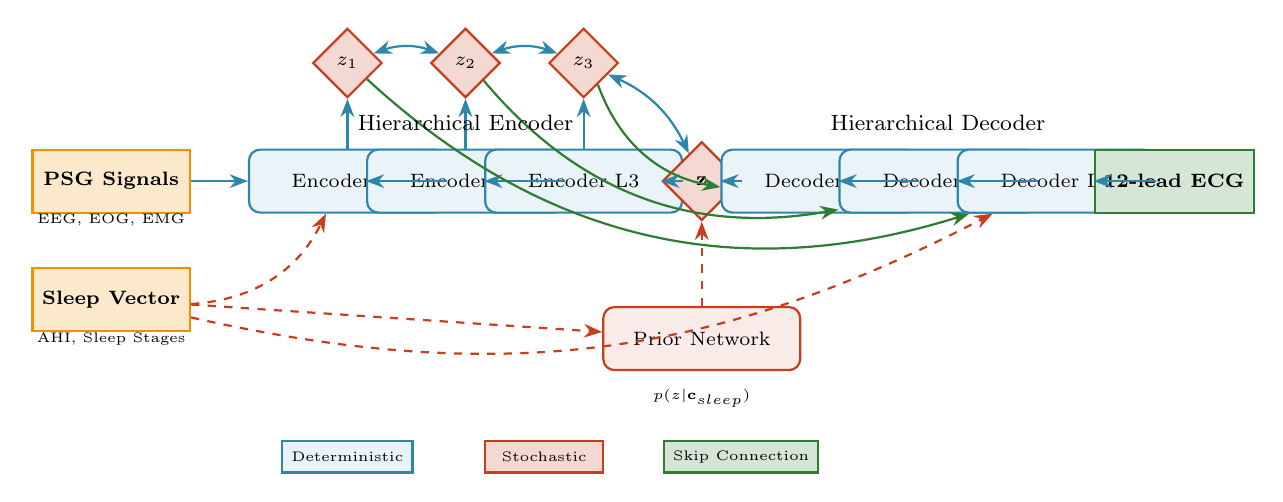
\begin{tikzpicture}[
    >=Stealth,
    % Define styles
    neuron/.style={circle, draw=black, thick, fill=white, minimum size=0.6cm},
    stochastic/.style={diamond, draw=tcairemred, thick, fill=tcairemred!20, minimum size=0.8cm},
    layer/.style={rectangle, draw=tcairemblue, thick, rounded corners, fill=tcairemblue!10, minimum width=2.5cm, minimum height=0.8cm},
    input/.style={rectangle, draw=tcairemorange, thick, fill=tcairemorange!20, minimum width=2cm, minimum height=0.8cm},
    output/.style={rectangle, draw=tcairemgreen, thick, fill=tcairemgreen!20, minimum width=2cm, minimum height=0.8cm},
    arrow/.style={->, thick, tcairemblue},
    bidirect/.style={<->, thick, tcairemblue},
    conditioning/.style={->, thick, tcairemred, dashed},
    % Font
    font=\scriptsize
]

% Input nodes
\node[input] (psg) at (-6, 0) {\textbf{PSG Signals}};
\node[input] (sleep) at (-6, -1.5) {\textbf{Sleep Vector}};
\node[font=\tiny] at (-6, -0.5) {EEG, EOG, EMG};
\node[font=\tiny] at (-6, -2) {AHI, Sleep Stages};

% Encoder layers (hierarchical)
\node[layer] (enc1) at (-3, 0) {Encoder L1};
\node[layer] (enc2) at (-1.5, 0) {Encoder L2};
\node[layer] (enc3) at (0, 0) {Encoder L3};

% Stochastic layers in encoder
\node[stochastic] (z3) at (0, 1.5) {$z_3$};
\node[stochastic] (z2) at (-1.5, 1.5) {$z_2$};
\node[stochastic] (z1) at (-3, 1.5) {$z_1$};

% Central latent representation
\node[stochastic, minimum size=1cm] (z) at (1.5, 0) {$\mathbf{z}$};

% Decoder layers (hierarchical)
\node[layer] (dec3) at (3, 0) {Decoder L3};
\node[layer] (dec2) at (4.5, 0) {Decoder L2};
\node[layer] (dec1) at (6, 0) {Decoder L1};

% Output
\node[output] (ecg) at (7.5, 0) {\textbf{12-lead ECG}};

% Prior network (conditional)
\node[layer, fill=tcairemred!10, draw=tcairemred] (prior) at (1.5, -2) {Prior Network};

% Connections - Encoder path
\draw[arrow] (psg) -- (enc1);
\draw[arrow] (enc1) -- (enc2);
\draw[arrow] (enc2) -- (enc3);
\draw[arrow] (enc3) -- (z);

% Stochastic connections from encoder
\draw[arrow] (enc1) -- (z1);
\draw[arrow] (enc2) -- (z2);
\draw[arrow] (enc3) -- (z3);

% Hierarchical dependencies
\draw[bidirect, bend left=20] (z1) to (z2);
\draw[bidirect, bend left=20] (z2) to (z3);
\draw[bidirect, bend left=20] (z3) to (z);

% Decoder path
\draw[arrow] (z) -- (dec3);
\draw[arrow] (dec3) -- (dec2);
\draw[arrow] (dec2) -- (dec1);
\draw[arrow] (dec1) -- (ecg);

% Conditioning paths
\draw[conditioning] (sleep) -- (prior);
\draw[conditioning] (prior) -- (z);
\draw[conditioning, bend right=30] (sleep) to (enc1);
\draw[conditioning, bend right=20] (sleep) to (dec1);

% Skip connections (residual)
\draw[arrow, tcairemgreen, bend right=30] (z3) to (dec3);
\draw[arrow, tcairemgreen, bend right=30] (z2) to (dec2);
\draw[arrow, tcairemgreen, bend right=30] (z1) to (dec1);

% Labels
\node[font=\footnotesize, above=0.1cm of enc2] {Hierarchical Encoder};
\node[font=\footnotesize, above=0.1cm of dec2] {Hierarchical Decoder};
\node[font=\tiny, below=0.1cm of prior] {$p(z|\mathbf{c}_{sleep})$};

% Legend boxes
\node[draw=tcairemblue, thick, fill=tcairemblue!10, minimum width=1.5cm, minimum height=0.4cm, font=\tiny] at (-3, -3.5) {Deterministic};
\node[draw=tcairemred, thick, fill=tcairemred!20, minimum width=1.5cm, minimum height=0.4cm, font=\tiny] at (-0.5, -3.5) {Stochastic};
\node[draw=tcairemgreen, thick, fill=tcairemgreen!20, minimum width=1.5cm, minimum height=0.4cm, font=\tiny] at (2, -3.5) {Skip Connection};

\end{tikzpicture}
}

\vspace{0.5em}
\begin{columns}[T,totalwidth=\linewidth]
  \column{0.48\linewidth}
    \colorbox{tcairemblue!15}{%
      \parbox{0.95\linewidth}{%
        \footnotesize\textcolor{tcairemblue}{\textbf{cNVAE-ECG core (kept)}}\\
        \tiny • 3-level hierarchical VAE structure\\
        \tiny • Bidirectional stochastic dependencies\\
        \tiny • Mixture-logistic output distribution}}
  \column{0.48\linewidth}
    \colorbox{tcairemred!15}{%
      \parbox{0.95\linewidth}{%
        \footnotesize\textcolor{tcairemred}{\textbf{Our extensions}}\\
        \tiny • PSG multi-channel input encoding\\
        \tiny • Sleep-conditioned prior network\\
        \tiny • Cross-modal skip connections}}
\end{columns}
\end{frame}


\begin{frame}{Proposed cNVAE-ECG Architecture}
  \centering
  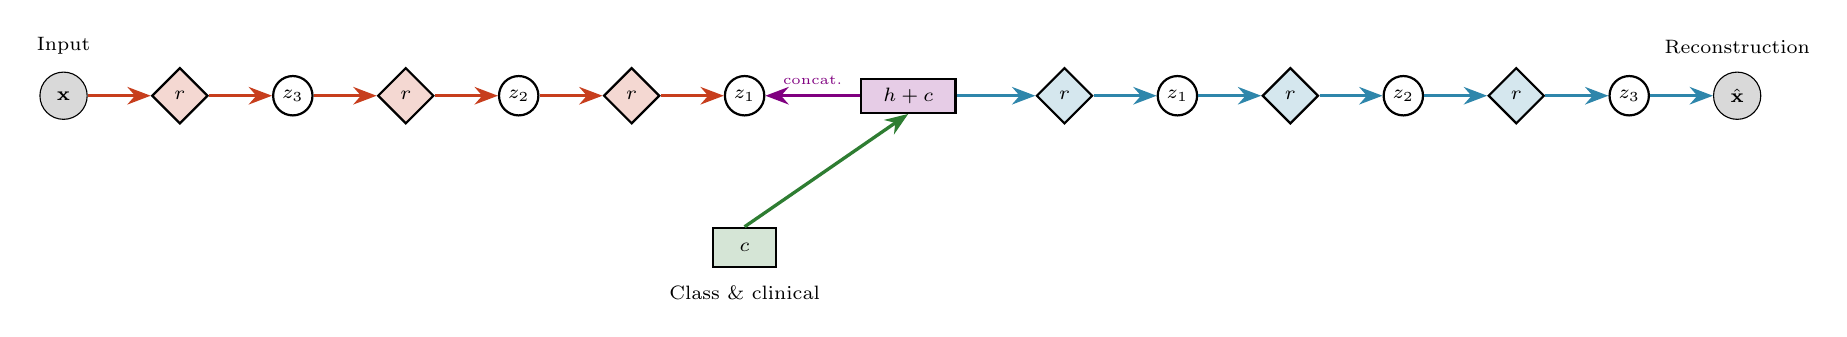
\begin{tikzpicture}[
      font=\scriptsize,
      >=Stealth,
      arr/.style={->, very thick},
      enc/.style={draw,diamond,thick,fill=tcairemred!20,minimum size=6mm},
      dec/.style={draw,diamond,thick,fill=tcairemblue!20,minimum size=6mm},
      plus/.style={draw,circle,thick,inner sep=0pt,minimum size=5mm},
      embed/.style={draw,rectangle,thick,fill=tcairemgreen!20,minimum height=5mm,minimum width=8mm}
    ]

    % Encoder (bottom-up)
    \node (x)    [draw,circle,fill=gray!30,minimum size=6mm] {$\mathbf{x}$};
    \node (r_e1) [enc, right=8mm of x]                     {$r$};
    \node (z_3)  [plus, right=8mm of r_e1]                  {$z_3$};
    \node (r_e2) [enc, right=8mm of z_3]                    {$r$};
    \node (z_2)  [plus, right=8mm of r_e2]                  {$z_2$};
    \node (r_e3) [enc, right=8mm of z_2]                    {$r$};
    \node (z_1)  [plus, right=8mm of r_e3]                  {$z_1$};

    % Arrows encoder
    \draw[arr,tcairemred] (x)    -- (r_e1);
    \draw[arr,tcairemred] (r_e1) -- (z_3);
    \draw[arr,tcairemred] (z_3)  -- (r_e2);
    \draw[arr,tcairemred] (r_e2) -- (z_2);
    \draw[arr,tcairemred] (z_2)  -- (r_e3);
    \draw[arr,tcairemred] (r_e3) -- (z_1);

    % Conditioning embedding
    \node (c)   [embed, below=14mm of z_1]               {$c$};
    \node (h)   [draw,rectangle,thick,fill=tcairempurple!20,minimum width=12mm,right=12mm of z_1]
                                                      {$h + c$};
    \draw[arr,tcairempurple] (h.west) -- node[above,font=\tiny]{concat.} (z_1.east);
    \draw[arr,tcairemgreen]   (c.north) -- (h.south);

    % Decoder (top-down)
    \node (r_d1) [dec, right=10mm of h]                    {$r$};
    \node (p_1)  [plus, right=8mm of r_d1]                 {$z_1$};
    \node (r_d2) [dec, right=8mm of p_1]                   {$r$};
    \node (p_2)  [plus, right=8mm of r_d2]                 {$z_2$};
    \node (r_d3) [dec, right=8mm of p_2]                   {$r$};
    \node (p_3)  [plus, right=8mm of r_d3]                 {$z_3$};
    \node (xhat) [draw,circle,fill=gray!30,minimum size=6mm,right=8mm of p_3]
                                                      {$\hat{\mathbf{x}}$};

    % Arrows decoder
    \draw[arr,tcairemblue] (h)    -- (r_d1);
    \draw[arr,tcairemblue] (r_d1) -- (p_1);
    \draw[arr,tcairemblue] (p_1)  -- (r_d2);
    \draw[arr,tcairemblue] (r_d2) -- (p_2);
    \draw[arr,tcairemblue] (p_2)  -- (r_d3);
    \draw[arr,tcairemblue] (r_d3) -- (p_3);
    \draw[arr,tcairemblue] (p_3)  -- (xhat);

    % Labels
    \node[above=1mm of x]    {Input};
    \node[above=1mm of xhat] {Reconstruction};
    \node[below=1mm of c]    {Class \& clinical};
  \end{tikzpicture}
\end{frame}
%--------------------------------------------------------------------

\begin{frame}{Our Cross-Modal Adaptation Methodology}
  \textbf{\textcolor{tcairemblue}{Mathematical Framework for PSG-to-ECG Reconstruction}}
  
  \vspace{0.3em}
  \textbf{\textcolor{tcairemgreen}{Original cNVAE-ECG Model:}}
  \begin{align}
  p(\mathbf{x}_{\text{ECG}} | \mathbf{c}_{\text{pathology}}) &= \int p(\mathbf{x}_{\text{ECG}} | \mathbf{z}) p(\mathbf{z} | \mathbf{c}_{\text{pathology}}) d\mathbf{z}
  \end{align}
  
  \textbf{\textcolor{tcairemred}{Our Adaptation for Cross-Modal Reconstruction:}}
  \begin{align}
  p(\mathbf{x}_{\text{ECG}} | \mathbf{x}_{\text{PSG}}, \mathbf{c}_{\text{sleep}}, \mathbf{s}) &= \int p(\mathbf{x}_{\text{ECG}} | \mathbf{z}) p(\mathbf{z} | \mathbf{x}_{\text{PSG}}, \mathbf{c}_{\text{sleep}}, \mathbf{s}) d\mathbf{z}
  \end{align}
  
  \textbf{\textcolor{tcairemblue}{Novel Loss Function Extension:}}
  \begin{align}
  \mathcal{L}_{\text{our}} &= \underbrace{\textcolor{tcairemblue}{\mathcal{L}_{\text{recon}}}}_{\text{ECG Fidelity (Original)}} + \underbrace{\textcolor{tcairemblue}{\mathcal{L}_{\text{KL}}}}_{\text{Regularization (Original)}} + \underbrace{\textcolor{tcairemred}{\mathcal{L}_{\text{sleep-cond}}}}_{\text{Sleep Conditioning (Novel)}}
  \end{align}
  
  where $\mathbf{x}_{\text{PSG}} \in \mathbb{R}^{7 \times T}$ (EEG, EOG, EMG, respiratory), $\mathbf{c}_{\text{sleep}} \in \mathbb{R}^{47}$ (clinical variables), $\mathbf{s}$ (sleep stage)

  \begin{columns}[T]
    \begin{column}{0.5\textwidth}
      \textbf{\textcolor{tcairemblue}{Preserved from Original}}
      \begin{itemize}
        \tiny
        \item Hierarchical VAE encoder/decoder architecture
        \item Multi-scale latent representation (3 scales)
        \item 12-lead ECG output generation
        \item Mixture of discretized logistic distributions
      \end{itemize}
    \end{column}
    \begin{column}{0.5\textwidth}
      \textbf{\textcolor{tcairemred}{Our Novel Adaptations}}
      \begin{itemize}
        \tiny
        \item PSG signal encoder replacing noise input
        \item Sleep clinical variable conditioning vectors
        \item Cross-modal attention mechanisms
        \item Sleep stage-aware latent conditioning
      \end{itemize}
    \end{column}
  \end{columns}
  
  \highlightbox[tcairemred]{Core Research Contribution: Feasibility study of adapting established ECG generation methods for cross-modal PSG-to-ECG reconstruction}
\end{frame}

\begin{frame}{Core Research Questions}
  
      \colorbox{tcairemblue!15}{\parbox{0.95\textwidth}{
    \large
    \textcolor{tcairemblue}{\textbf{Can we successfully replace random noise input with PSG signals in the cNVAE-ECG architecture?}}\\
  }}
  
      \colorbox{tcairemorange!15}{\parbox{0.95\textwidth}{
    \large
    \textcolor{tcairemorange}{\textbf{Do basic sleep clinical variables (AHI, sleep stages) improve reconstruction quality over PSG signals alone?}}\\
}}
    \colorbox{tcairemgreen!15}{\parbox{0.95\textwidth}{
    \large
    \textcolor{tcairemgreen}{\textbf{What are the fundamental limitations preventing higher reconstruction quality?}}


  }}

\end{frame}








%---------------------------------------------------------------

%===================================================================
% 6 ▸  Data Pipeline & Normalisation
%===================================================================
\begin{frame}{Data Pipeline – From Raw PSG to Model‑ready Tensors}
\begin{block}{Stage A – Window Extraction}
\small EDF → 30‑s windows → resample to 128 Hz → band‑pass (0.5–40\,\mathrm{Hz}\text{ ECG}\; 0.1–20\,\mathrm{Hz}\text{ PSG})
\end{block}

\begin{block}{Stage B – \textcolor{tcairemred}{\textbf{Global z‑score}} (NEW)}
\small Compute per‑channel $(\mu,\sigma)$ using $(\sim100\,\text{k})$ train windows → $\tilde{x} = \frac{x-\mu}{\sigma+10^{-8}}$
\vspace{0.2em}
Replaces previous min‑max (1–99 pc) scaling → consistent amplitude across modalities.
\end{block}

\begin{block}{Stage C – Augmentation (train only)}
\small Time‑shift, amplitude‑jitter, channel dropout, additive noise (controlled via YAML config).
\end{block}

\highlightbox[tcairempurple]{Sanity check: disable Stage C + β=0 to verify reconstruction path}
\end{frame}

%===================================================================
% 7 ▸  Single‑Batch Overfit Protocol
%===================================================================
\begin{frame}{"Single‑Batch" Overfit Sanity Test}
\begin{columns}[T]
\begin{column}{0.55\textwidth}
\begin{enumerate}\itemsep0.25em
\item Turn \textbf{off} augmentation
\item Freeze KL → $\beta=0$
\item Select $N=32$ windows (one mini‑batch)
\item Train 800 epochs, lr = 1e‑3
\end{enumerate}

\vspace{0.6em}
\textbf{Expected}\,: NELBO $\downarrow$ $(<50)$ and $|r| \to1$.
\end{column}

\begin{column}{0.43\textwidth}
\centering
\includegraphics[width=\linewidth]{protocol_diagram.png}
\tiny Fig: training loop instrumentation
\end{column}
\end{columns}
\end{frame}

%===================================================================
% 8 ▸  Preliminary Observation (pre‑fix)
%===================================================================
\begin{frame}{Pre‑Normalisation Baseline – Why Scaling Matters}
\begin{columns}[T]
\begin{column}{0.55\textwidth}
\begin{itemize}\itemsep0.3em
\item Test \textbf{NELBO} ≈ \textbf{8 942}; (min‑max scaling)
\item Pearson r (lead II) ≈ \textbf{−0.001}
\item Decoder collapsed → nearly \emph{flat} output
\item Hypothesis: inconsistent amplitude across channels inhibits likelihood learning.
\end{itemize}
\end{column}

\begin{column}{0.42\textwidth}
\centering
\includegraphics[width=\linewidth]{ecg_recon.png}
\tiny ECG Recon– Tiny snippet (blue GT, orange pred)
\end{column}
\end{columns}
\highlightbox[tcairemred]{Fix: global z‑score + β=0 single‑batch overfit $\Rightarrow$ running}
\end{frame}

%===================================================================
% 9 ▸  Experiment Status
%===================================================================
\begin{frame}{Current Status \& Next 2 Weeks}
\begin{columns}[T]
\begin{column}{0.6\textwidth}
\textbf{In progress}
\begin{itemize}\itemsep0.25em
\item Global‑normalised single‑batch run (GPU A100 – ETA $\sim4 h$)
\item TensorBoard live tracking (loss \& r)
\end{itemize}

\vspace{0.4em}
\textbf{Next Steps}
\begin{itemize}\itemsep0.25em
\item Re‑enable KL annealing (β‑schedule)
\item Curriculum: add augmentation → full dataset
\item Ablation: prior MLP vs. no sleep conditioning
\item Evaluation: arrhythmia detection metric (AUROC) on reconstructed vs. recorded ECG
\end{itemize}
\end{column}

\begin{column}{0.38\textwidth}
\centering
\includegraphics[width=\linewidth]{roadmap.png}
\tiny Milestone Gantt (Aug–Dec 2025)
\end{column}
\end{columns}
\end{frame}






\iffalse % condensed: skipping research questions and subsequent hypothesis slides

\begin{frame}{Simple Hypotheses}
  \textbf{\textcolor{tcairemblue}{\Large What We Think Might Work}}
  
  \vspace{1.5em}
  \textbf{\textcolor{tcairemgreen}{\large H1: Basic Information Transfer}}
      \begin{itemize}
    \large
    \item PSG signals contain \textbf{some cardiac information} that can be extracted
    \vspace{0.5em}
    \item Sleep stages and AHI will \textbf{help} the reconstruction process
      \end{itemize}
      
  \vspace{1.5em}
  \textbf{\textcolor{tcairemorange}{\large H2: Stage-Dependent Performance}}
      \begin{itemize}
    \large
    \item Some sleep stages (e.g., REM) might be \textbf{easier to reconstruct} than others
    \vspace{0.5em}
    \item Patients with \textbf{severe sleep apnea} might show stronger PSG-ECG coupling
      \end{itemize}
      
  \vspace{1.5em}
  \colorbox{tcairemblue!15}{\parbox{0.95\textwidth}{
    \large
    \textcolor{tcairemblue}{\textbf{Reality Check}}\\
    \vspace{0.5em}
    \normalsize
    These are educated guesses. We might be completely wrong, and that's okay - 
    that's what Phase 1-2 is for.
  }}
\end{frame}


%===================================================================%
%  T-CAIREM Mid-Term presentation   ––  Clean compile version
%===================================================================%
\documentclass[aspectratio=169,11pt]{beamer}

% ------------------------------------------------------------------
%  GLOBAL THEME  &  COLORS
% ------------------------------------------------------------------
\usetheme{Madrid}
\usecolortheme{beaver}

% brand colours
\definecolor{tcairemblue}{RGB}{46,134,171}
\definecolor{tcairemred}{RGB}{199,62,29}
\definecolor{tcairemorange}{RGB}{241,143,1}
\definecolor{tcairempurple}{RGB}{128,0,128}
\definecolor{tcairemgreen}{RGB}{46,125,50}

\setbeamercolor{structure}{fg=tcairemblue}
\setbeamercolor{frametitle}{bg=tcairemblue,fg=white}

% ------------------------------------------------------------------
%  HEADER / FOOTER
% ------------------------------------------------------------------
\setbeamertemplate{headline}{%
  \begin{beamercolorbox}[ht=5ex,dp=1.5ex]{section in head/foot}
    \hspace{1em}
\includegraphics[height=4.5ex]{SRI_logo.png}\hfill
    
\includegraphics[height=5ex]{TCAIREM_logo.jpg}\hspace{1em}
  \end{beamercolorbox}
}
\setbeamertemplate{footline}{%
  \begin{beamercolorbox}[ht=2.5ex,dp=1ex,center]{author in head/foot}
    \insertshortauthor\hspace{2em}\insertshortinstitute\hspace{4em}
    \insertframenumber{} / \inserttotalframenumber
  \end{beamercolorbox}
}

% ------------------------------------------------------------------
%  BLOCK COLOURS / HIGHLIGHT MACRO
% ------------------------------------------------------------------
\setbeamercolor{block title}{bg=tcairemblue,fg=white}
\setbeamercolor{block body}{bg=tcairemblue!15,fg=black}
\setbeamercolor{block title example}{bg=tcairemorange,fg=white}
\setbeamercolor{block body example}{bg=tcairemorange!15,fg=black}
\setbeamercolor{block title alerted}{bg=tcairemred,fg=white}
\setbeamercolor{block body alerted}{bg=tcairemred!15,fg=black}

\newcommand{\highlightbox}[2][tcairemred]{%
  \begin{center}
    \colorbox{#1!20}{\parbox{0.9\textwidth}{\centering\textcolor{#1}{\textbf{#2}}}}
  \end{center}}

% ------------------------------------------------------------------
%  PACKAGES
% ------------------------------------------------------------------
\usepackage[utf8]{inputenc}
\usepackage[T1]{fontenc}
\usepackage{textcomp}
\usepackage{graphicx}
\usepackage{amsmath,amssymb}
\usepackage{booktabs}
\usepackage{hyperref}

% TikZ ── load *once*, after package
\usepackage{tikz}
\usetikzlibrary{arrows.meta,calc,positioning,shapes.geometric}

% ------------------------------------------------------------------
%  DOC INFO
% ------------------------------------------------------------------
\title[T-CAIREM Mid-Term]{Application of Deep Hierarchical VAE for ECG Reconstruction}
\author{Mithun Manivannan, MSc (c)}
\institute[T-CAIREM]{Schulich Heart Program \\ Sunnybrook Health Sciences Centre}
\date{July 9, 2025}

%===================================================================%
\begin{document}

%--------------------------------------------------------------------
\begin{frame}
  \titlepage

  \vspace{-3.5em}
  \begin{columns}[c]
    \column{0.3\textwidth}\centering
\includegraphics[height=2.2cm]{SRI_logo.png}
    \column{0.4\textwidth}
    \column{0.3\textwidth}\centering
\includegraphics[height=2.2cm]{TCAIREM_logo.jpg}
  \end{columns}
\end{frame}


\begin{frame}{Clinical Problem: Sleep-Cardiac Monitoring Gap}

  \begin{columns}[T]
    \begin{column}{0.5\textwidth}
      \colorbox{tcairemred!15}{\parbox{0.95\textwidth}{
        \small
        \textcolor{tcairemred}{\textbf{Established, but not well understood }}\\
        \vspace{0.3em}
        • \textbf{80\%} of sleep apnea patients have undiagnosed cardiac arrhythmias\\
        \vspace{0.2em}
        • \textbf{45\%} increase in cardiac events during specific sleep stages\\
      }}
      
      \vspace{0.5em}
      \colorbox{tcairemorange!15}{\parbox{0.95\textwidth}{
        \small
        \textcolor{tcairemorange}{\textbf{Current Diagnostic Limitations}}\\
        \vspace{0.3em}
        • PSG studies lack continuous cardiac monitoring\\
        \vspace{0.2em}
      }}
    \end{column}
    \begin{column}{0.5\textwidth}
      \colorbox{tcairemgreen!15}{\parbox{0.95\textwidth}{
        \small
        \textcolor{tcairemgreen}{\textbf{Treatment Optimization Barriers}}\\
        \vspace{0.3em}
        • CPAP therapy cardiac impact poorly quantified\\
        \vspace{0.2em}
        • Sleep medication cardiac effects undermonitored\\
        \vspace{0.2em}
        • Individual treatment response highly variable\\
        \vspace{0.2em}
        • No personalized risk stratification tools
      }}
      
      \vspace{0.5em}
      \colorbox{tcairemblue!15}{\parbox{0.95\textwidth}{
        \small
        \textcolor{tcairemblue}{\textbf{Workflow Inefficiencies}}\\
        \vspace{0.3em}
        • Limited simultaneous PSG-ECG monitoring\\
        \vspace{0.2em}
        • \textbf{3x} cost increase for comprehensive assessment
      }}
    \end{column}
  \end{columns}
  
  \begin{center}
    \highlightbox[tcairempurple]{Need: Integrated sleep-cardiac monitoring solution for comprehensive patient assessment}
  \end{center}
\end{frame}

\begin{frame}{Technical Challenges in Cross-Modal Modeling}  
    \textbf{\textcolor{tcairemblue}{Why PSG-to-ECG Reconstruction is Challenging}}

  \begin{columns}[T]
    \begin{column}{0.5\textwidth}
      \textbf{\textcolor{tcairemred}{Signal Processing }}
      \begin{itemize}
        \item  PSG-ECG signals have different temporal dynamics during sleep transitions
        \vspace{0.3em}

        \item  Sleep phenomena span microseconds to hours
      \end{itemize}
    \end{column}
    \begin{column}{0.5\textwidth}
      \textbf{\textcolor{tcairemorange}{Individual Variability}}
      \begin{itemize}
        \item Physiological Coupling
        \vspace{0.3em}
        \item Comorbidity Effects 
        \vspace{0.3em}
        \item Medication Interactions
        \vspace{0.3em}
        \item Demographic Factors
      \end{itemize}
    \end{column}
  \end{columns}
    
  \vspace{0.5em}
  \highlightbox[tcairemgreen]{Goal: Develop robust cross-modal models that work across diverse patients and clinical environments}
\end{frame}





\begin{frame}{Existing Methods}
  \begin{columns}[T]
    \begin{column}{0.48\textwidth}
      \begin{itemize}
        %—- Emphasise the move from GANs to VAEs
        \item Transition from \textbf{GAN-based} ECG generators to \textbf{Variational Autoencoders (VAEs)}
        %—- Cite the paper you provided
        \item \textbf{cNVAE-ECG} \tiny(Sviridov \& Egorov, 2025)\normalsize: conditional \emph{hierarchical} VAE
        %—- Interpretability bullet
        \item Multi-scale latent hierarchy disentangles\\[-0.3em]
              \hspace{1em}• beat-level morphology (P, QRS, T)\\[-0.3em]
              \hspace{1em}• pathology-level context
        %—- Likelihood & uncertainty
        \item Explicit likelihood and latent traversals $\Rightarrow$ clinical interpretability \& uncertainty quantification
        %—- Brief performance reference
        \item +2 \% AUROC vs.\ state-of-the-art GANs on PTB-XL
      \end{itemize}

      \highlightbox[tcairemred]{Interpretability: hierarchical VAEs map distinct latent layers to ECG waves and rhythm context.}
    \end{column}

    \begin{column}{0.52\textwidth}
      \begin{center}
        \includegraphics[width=1.0\textwidth,height=1.2\textheight,keepaspectratio]{cnvae-ecg_arch.jpeg}
      \end{center}
    \end{column}
  \end{columns}
\end{frame}

%--------------------------------------------------------------------
%--------------------------------------------------------------------
\begin{frame}{Proposed architecture — cNVAE-ECG adapted for PSG \& sleep context}
\centering
\vspace{-0.5em}
\resizebox{0.95\linewidth}{!}{%
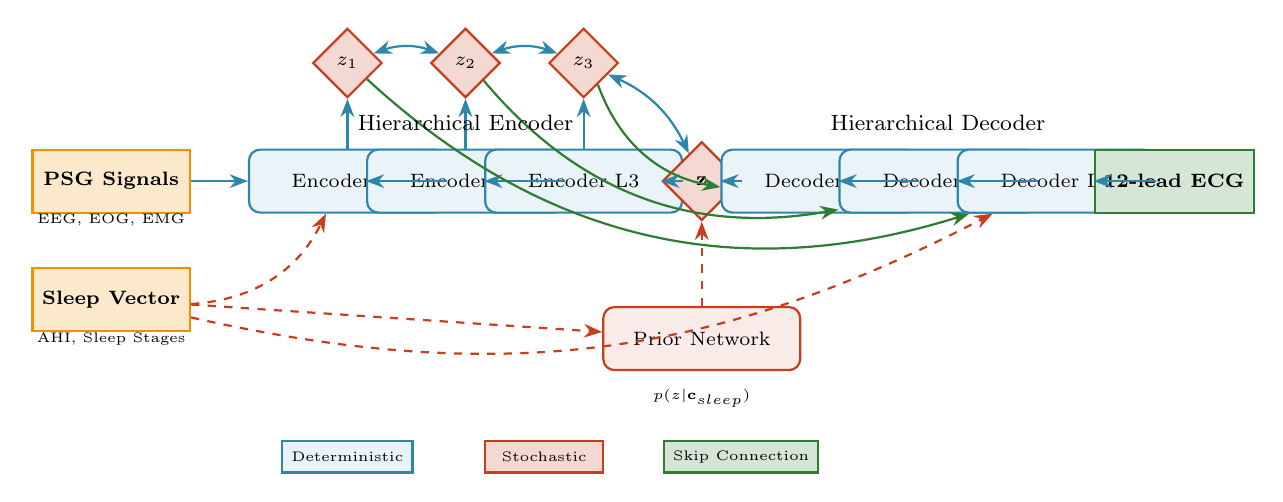
\begin{tikzpicture}[
    >=Stealth,
    % Define styles
    neuron/.style={circle, draw=black, thick, fill=white, minimum size=0.6cm},
    stochastic/.style={diamond, draw=tcairemred, thick, fill=tcairemred!20, minimum size=0.8cm},
    layer/.style={rectangle, draw=tcairemblue, thick, rounded corners, fill=tcairemblue!10, minimum width=2.5cm, minimum height=0.8cm},
    input/.style={rectangle, draw=tcairemorange, thick, fill=tcairemorange!20, minimum width=2cm, minimum height=0.8cm},
    output/.style={rectangle, draw=tcairemgreen, thick, fill=tcairemgreen!20, minimum width=2cm, minimum height=0.8cm},
    arrow/.style={->, thick, tcairemblue},
    bidirect/.style={<->, thick, tcairemblue},
    conditioning/.style={->, thick, tcairemred, dashed},
    % Font
    font=\scriptsize
]

% Input nodes
\node[input] (psg) at (-6, 0) {\textbf{PSG Signals}};
\node[input] (sleep) at (-6, -1.5) {\textbf{Sleep Vector}};
\node[font=\tiny] at (-6, -0.5) {EEG, EOG, EMG};
\node[font=\tiny] at (-6, -2) {AHI, Sleep Stages};

% Encoder layers (hierarchical)
\node[layer] (enc1) at (-3, 0) {Encoder L1};
\node[layer] (enc2) at (-1.5, 0) {Encoder L2};
\node[layer] (enc3) at (0, 0) {Encoder L3};

% Stochastic layers in encoder
\node[stochastic] (z3) at (0, 1.5) {$z_3$};
\node[stochastic] (z2) at (-1.5, 1.5) {$z_2$};
\node[stochastic] (z1) at (-3, 1.5) {$z_1$};

% Central latent representation
\node[stochastic, minimum size=1cm] (z) at (1.5, 0) {$\mathbf{z}$};

% Decoder layers (hierarchical)
\node[layer] (dec3) at (3, 0) {Decoder L3};
\node[layer] (dec2) at (4.5, 0) {Decoder L2};
\node[layer] (dec1) at (6, 0) {Decoder L1};

% Output
\node[output] (ecg) at (7.5, 0) {\textbf{12-lead ECG}};

% Prior network (conditional)
\node[layer, fill=tcairemred!10, draw=tcairemred] (prior) at (1.5, -2) {Prior Network};

% Connections - Encoder path
\draw[arrow] (psg) -- (enc1);
\draw[arrow] (enc1) -- (enc2);
\draw[arrow] (enc2) -- (enc3);
\draw[arrow] (enc3) -- (z);

% Stochastic connections from encoder
\draw[arrow] (enc1) -- (z1);
\draw[arrow] (enc2) -- (z2);
\draw[arrow] (enc3) -- (z3);

% Hierarchical dependencies
\draw[bidirect, bend left=20] (z1) to (z2);
\draw[bidirect, bend left=20] (z2) to (z3);
\draw[bidirect, bend left=20] (z3) to (z);

% Decoder path
\draw[arrow] (z) -- (dec3);
\draw[arrow] (dec3) -- (dec2);
\draw[arrow] (dec2) -- (dec1);
\draw[arrow] (dec1) -- (ecg);

% Conditioning paths
\draw[conditioning] (sleep) -- (prior);
\draw[conditioning] (prior) -- (z);
\draw[conditioning, bend right=30] (sleep) to (enc1);
\draw[conditioning, bend right=20] (sleep) to (dec1);

% Skip connections (residual)
\draw[arrow, tcairemgreen, bend right=30] (z3) to (dec3);
\draw[arrow, tcairemgreen, bend right=30] (z2) to (dec2);
\draw[arrow, tcairemgreen, bend right=30] (z1) to (dec1);

% Labels
\node[font=\footnotesize, above=0.1cm of enc2] {Hierarchical Encoder};
\node[font=\footnotesize, above=0.1cm of dec2] {Hierarchical Decoder};
\node[font=\tiny, below=0.1cm of prior] {$p(z|\mathbf{c}_{sleep})$};

% Legend boxes
\node[draw=tcairemblue, thick, fill=tcairemblue!10, minimum width=1.5cm, minimum height=0.4cm, font=\tiny] at (-3, -3.5) {Deterministic};
\node[draw=tcairemred, thick, fill=tcairemred!20, minimum width=1.5cm, minimum height=0.4cm, font=\tiny] at (-0.5, -3.5) {Stochastic};
\node[draw=tcairemgreen, thick, fill=tcairemgreen!20, minimum width=1.5cm, minimum height=0.4cm, font=\tiny] at (2, -3.5) {Skip Connection};

\end{tikzpicture}
}

\vspace{0.5em}
\begin{columns}[T,totalwidth=\linewidth]
  \column{0.48\linewidth}
    \colorbox{tcairemblue!15}{%
      \parbox{0.95\linewidth}{%
        \footnotesize\textcolor{tcairemblue}{\textbf{cNVAE-ECG core (kept)}}\\
        \tiny • 3-level hierarchical VAE structure\\
        \tiny • Bidirectional stochastic dependencies\\
        \tiny • Mixture-logistic output distribution}}
  \column{0.48\linewidth}
    \colorbox{tcairemred!15}{%
      \parbox{0.95\linewidth}{%
        \footnotesize\textcolor{tcairemred}{\textbf{Our extensions}}\\
        \tiny • PSG multi-channel input encoding\\
        \tiny • Sleep-conditioned prior network\\
        \tiny • Cross-modal skip connections}}
\end{columns}
\end{frame}


\begin{frame}{Proposed cNVAE-ECG Architecture}
  \centering
  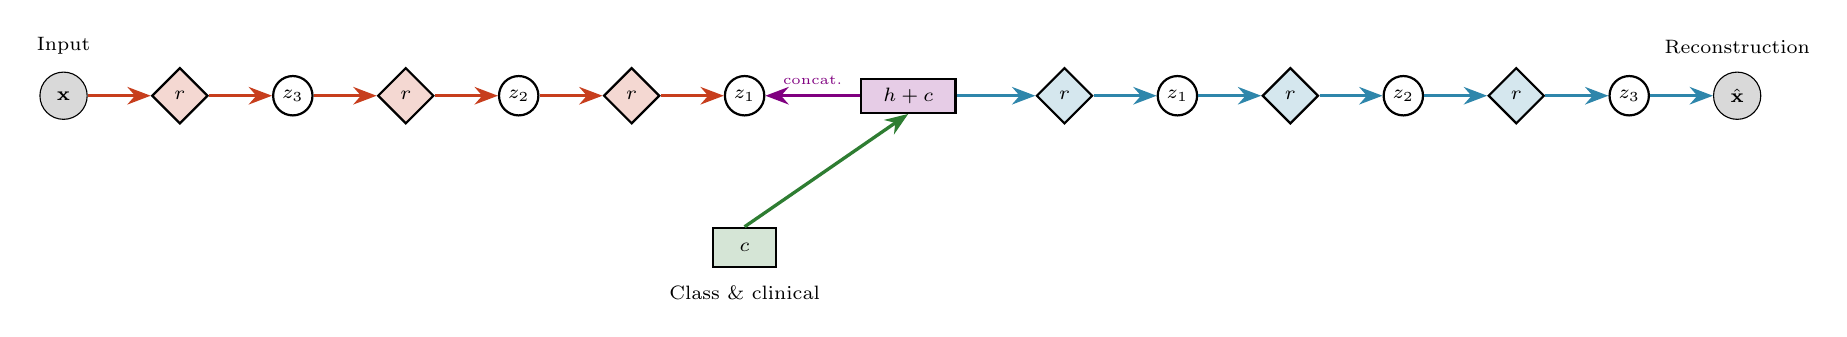
\begin{tikzpicture}[
      font=\scriptsize,
      >=Stealth,
      arr/.style={->, very thick},
      enc/.style={draw,diamond,thick,fill=tcairemred!20,minimum size=6mm},
      dec/.style={draw,diamond,thick,fill=tcairemblue!20,minimum size=6mm},
      plus/.style={draw,circle,thick,inner sep=0pt,minimum size=5mm},
      embed/.style={draw,rectangle,thick,fill=tcairemgreen!20,minimum height=5mm,minimum width=8mm}
    ]

    % Encoder (bottom-up)
    \node (x)    [draw,circle,fill=gray!30,minimum size=6mm] {$\mathbf{x}$};
    \node (r_e1) [enc, right=8mm of x]                     {$r$};
    \node (z_3)  [plus, right=8mm of r_e1]                  {$z_3$};
    \node (r_e2) [enc, right=8mm of z_3]                    {$r$};
    \node (z_2)  [plus, right=8mm of r_e2]                  {$z_2$};
    \node (r_e3) [enc, right=8mm of z_2]                    {$r$};
    \node (z_1)  [plus, right=8mm of r_e3]                  {$z_1$};

    % Arrows encoder
    \draw[arr,tcairemred] (x)    -- (r_e1);
    \draw[arr,tcairemred] (r_e1) -- (z_3);
    \draw[arr,tcairemred] (z_3)  -- (r_e2);
    \draw[arr,tcairemred] (r_e2) -- (z_2);
    \draw[arr,tcairemred] (z_2)  -- (r_e3);
    \draw[arr,tcairemred] (r_e3) -- (z_1);

    % Conditioning embedding
    \node (c)   [embed, below=14mm of z_1]               {$c$};
    \node (h)   [draw,rectangle,thick,fill=tcairempurple!20,minimum width=12mm,right=12mm of z_1]
                                                      {$h + c$};
    \draw[arr,tcairempurple] (h.west) -- node[above,font=\tiny]{concat.} (z_1.east);
    \draw[arr,tcairemgreen]   (c.north) -- (h.south);

    % Decoder (top-down)
    \node (r_d1) [dec, right=10mm of h]                    {$r$};
    \node (p_1)  [plus, right=8mm of r_d1]                 {$z_1$};
    \node (r_d2) [dec, right=8mm of p_1]                   {$r$};
    \node (p_2)  [plus, right=8mm of r_d2]                 {$z_2$};
    \node (r_d3) [dec, right=8mm of p_2]                   {$r$};
    \node (p_3)  [plus, right=8mm of r_d3]                 {$z_3$};
    \node (xhat) [draw,circle,fill=gray!30,minimum size=6mm,right=8mm of p_3]
                                                      {$\hat{\mathbf{x}}$};

    % Arrows decoder
    \draw[arr,tcairemblue] (h)    -- (r_d1);
    \draw[arr,tcairemblue] (r_d1) -- (p_1);
    \draw[arr,tcairemblue] (p_1)  -- (r_d2);
    \draw[arr,tcairemblue] (r_d2) -- (p_2);
    \draw[arr,tcairemblue] (p_2)  -- (r_d3);
    \draw[arr,tcairemblue] (r_d3) -- (p_3);
    \draw[arr,tcairemblue] (p_3)  -- (xhat);

    % Labels
    \node[above=1mm of x]    {Input};
    \node[above=1mm of xhat] {Reconstruction};
    \node[below=1mm of c]    {Class \& clinical};
  \end{tikzpicture}
\end{frame}
%--------------------------------------------------------------------

\begin{frame}{Our Cross-Modal Adaptation Methodology}
  \textbf{\textcolor{tcairemblue}{Mathematical Framework for PSG-to-ECG Reconstruction}}
  
  \vspace{0.3em}
  \textbf{\textcolor{tcairemgreen}{Original cNVAE-ECG Model:}}
  \begin{align}
  p(\mathbf{x}_{\text{ECG}} | \mathbf{c}_{\text{pathology}}) &= \int p(\mathbf{x}_{\text{ECG}} | \mathbf{z}) p(\mathbf{z} | \mathbf{c}_{\text{pathology}}) d\mathbf{z}
  \end{align}
  
  \textbf{\textcolor{tcairemred}{Our Adaptation for Cross-Modal Reconstruction:}}
  \begin{align}
  p(\mathbf{x}_{\text{ECG}} | \mathbf{x}_{\text{PSG}}, \mathbf{c}_{\text{sleep}}, \mathbf{s}) &= \int p(\mathbf{x}_{\text{ECG}} | \mathbf{z}) p(\mathbf{z} | \mathbf{x}_{\text{PSG}}, \mathbf{c}_{\text{sleep}}, \mathbf{s}) d\mathbf{z}
  \end{align}
  
  \textbf{\textcolor{tcairemblue}{Novel Loss Function Extension:}}
  \begin{align}
  \mathcal{L}_{\text{our}} &= \underbrace{\textcolor{tcairemblue}{\mathcal{L}_{\text{recon}}}}_{\text{ECG Fidelity (Original)}} + \underbrace{\textcolor{tcairemblue}{\mathcal{L}_{\text{KL}}}}_{\text{Regularization (Original)}} + \underbrace{\textcolor{tcairemred}{\mathcal{L}_{\text{sleep-cond}}}}_{\text{Sleep Conditioning (Novel)}}
  \end{align}
  
  where $\mathbf{x}_{\text{PSG}} \in \mathbb{R}^{7 \times T}$ (EEG, EOG, EMG, respiratory), $\mathbf{c}_{\text{sleep}} \in \mathbb{R}^{47}$ (clinical variables), $\mathbf{s}$ (sleep stage)

  \begin{columns}[T]
    \begin{column}{0.5\textwidth}
      \textbf{\textcolor{tcairemblue}{Preserved from Original}}
      \begin{itemize}
        \tiny
        \item Hierarchical VAE encoder/decoder architecture
        \item Multi-scale latent representation (3 scales)
        \item 12-lead ECG output generation
        \item Mixture of discretized logistic distributions
      \end{itemize}
    \end{column}
    \begin{column}{0.5\textwidth}
      \textbf{\textcolor{tcairemred}{Our Novel Adaptations}}
      \begin{itemize}
        \tiny
        \item PSG signal encoder replacing noise input
        \item Sleep clinical variable conditioning vectors
        \item Cross-modal attention mechanisms
        \item Sleep stage-aware latent conditioning
      \end{itemize}
    \end{column}
  \end{columns}
  
  \highlightbox[tcairemred]{Core Research Contribution: Feasibility study of adapting established ECG generation methods for cross-modal PSG-to-ECG reconstruction}
\end{frame}

\begin{frame}{Core Research Questions}
  
      \colorbox{tcairemblue!15}{\parbox{0.95\textwidth}{
    \large
    \textcolor{tcairemblue}{\textbf{Can we successfully replace random noise input with PSG signals in the cNVAE-ECG architecture?}}\\
  }}
  
      \colorbox{tcairemorange!15}{\parbox{0.95\textwidth}{
    \large
    \textcolor{tcairemorange}{\textbf{Do basic sleep clinical variables (AHI, sleep stages) improve reconstruction quality over PSG signals alone?}}\\
}}
    \colorbox{tcairemgreen!15}{\parbox{0.95\textwidth}{
    \large
    \textcolor{tcairemgreen}{\textbf{What are the fundamental limitations preventing higher reconstruction quality?}}


  }}

\end{frame}


\iffalse % condensed: skipping research questions and subsequent hypothesis slides

\begin{frame}{Simple Hypotheses}
  \textbf{\textcolor{tcairemblue}{\Large What We Think Might Work}}
  
  \vspace{1.5em}
  \textbf{\textcolor{tcairemgreen}{\large H1: Basic Information Transfer}}
      \begin{itemize}
    \large
    \item PSG signals contain \textbf{some cardiac information} that can be extracted
    \vspace{0.5em}
    \item Sleep stages and AHI will \textbf{help} the reconstruction process
      \end{itemize}
      
  \vspace{1.5em}
  \textbf{\textcolor{tcairemorange}{\large H2: Stage-Dependent Performance}}
      \begin{itemize}
    \large
    \item Some sleep stages (e.g., REM) might be \textbf{easier to reconstruct} than others
    \vspace{0.5em}
    \item Patients with \textbf{severe sleep apnea} might show stronger PSG-ECG coupling
      \end{itemize}
      
  \vspace{1.5em}
  \colorbox{tcairemblue!15}{\parbox{0.95\textwidth}{
    \large
    \textcolor{tcairemblue}{\textbf{Reality Check}}\\
    \vspace{0.5em}
    \normalsize
    These are educated guesses. We might be completely wrong, and that's okay - 
    that's what Phase 1-2 is for.
  }}
\end{frame}





\begin{frame}{Clinical Hypotheses: Physiological Mechanisms}
  \textbf{\textcolor{tcairemred}{\large H3: Physiological Coupling Mechanisms}}
  
  \vspace{0.5em}
      \begin{itemize}
    \large
    \item \textbf{Autonomic tone changes} will be detectable 30-60s before visible in ECG
    
    \vspace{0.5em}
    \item \textbf{Respiratory effort bands} will predict cardiac preload changes
    
    \vspace{0.5em}
    \item \textbf{Sleep stage transitions} will show predictable cardiac adaptation patterns
      \end{itemize}
      
  \vspace{1em}
  \textbf{\textcolor{tcairemblue}{\large H4: Clinical Validation Thresholds}}
  
  \vspace{0.5em}
      \begin{itemize}
    \large
    \item Reconstruction quality \textbf{r > 0.75} required for clinical arrhythmia detection
    
    \vspace{0.5em}
    \item \textbf{Individual adaptation} essential for patients with >3 comorbidities
    
    \vspace{0.5em}
    \item \textbf{Sleep-stage aware models} will improve accuracy by 15-25\% over naive approaches
      \end{itemize}
\end{frame}

\begin{frame}{Immediate Clinical Applications}
  \textbf{\textcolor{tcairemblue}{\Large Clinical Impact Areas}}
  
  \vspace{1em}
      \colorbox{tcairemgreen!15}{\parbox{0.95\textwidth}{
    \large
        \textcolor{tcairemgreen}{\textbf{Remote Cardiac Monitoring}}\\
    \vspace{0.5em}
    \normalsize
        • Enable ECG estimation during routine sleep studies\\
    \vspace{0.2em}
        • Continuous cardiac assessment without additional leads\\
    \vspace{0.2em}
        • Reduced patient burden and equipment complexity
      }}
      
  \vspace{0.8em}
      \colorbox{tcairemorange!15}{\parbox{0.95\textwidth}{
    \large
        \textcolor{tcairemorange}{\textbf{Sleep-Cardiac Comorbidity Assessment}}\\
    \vspace{0.5em}
    \normalsize
        • Identify cardiac arrhythmias during specific sleep stages\\
    \vspace{0.2em}
        • Quantify sleep's impact on cardiac health markers\\
    \vspace{0.2em}
        • Early detection of sleep-related cardiac issues
      }}
      
  \vspace{0.8em}
      \colorbox{tcairemred!15}{\parbox{0.95\textwidth}{
    \large
        \textcolor{tcairemred}{\textbf{Treatment Optimization}}\\
    \vspace{0.5em}
    \normalsize
        • CPAP therapy cardiac impact assessment\\
    \vspace{0.2em}
        • Sleep medication cardiac side effect monitoring\\
    \vspace{0.2em}
        • Personalized treatment recommendation systems
      }}
\end{frame}




\begin{frame}{Realistic Implementation Plan}
  \textbf{\textcolor{tcairemblue}{\Large Focus on Phase 1-2: Proof of Concept}}
  
  \vspace{1em}
  \colorbox{tcairemgreen!15}{\parbox{0.95\textwidth}{
    \large
    \textcolor{tcairemgreen}{\textbf{Phase 1: Basic Adaptation (Months 1-2)}}\\
    \vspace{0.8em}
    \normalsize
    • Get PSG signals feeding into cNVAE-ECG architecture\\
    \vspace{0.3em}
    • Replace noise input with simple PSG signal encoder\\  
    \vspace{0.3em}
    • See if the model can train without crashing\\
    \vspace{0.3em}
    • \textbf{Success:} Any positive correlation (r > 0.2) between output and real ECG
  }}
  
  \vspace{0.8em}
  \colorbox{tcairemorange!15}{\parbox{0.95\textwidth}{
    \large
    \textcolor{tcairemorange}{\textbf{Phase 2: Add Sleep Variables (Months 3-4)}}\\
    \vspace{0.8em}
    \normalsize
    • Add AHI and basic sleep stage information as conditioning\\
    \vspace{0.3em}
    • Test if sleep context helps reconstruction quality\\
    \vspace{0.3em}
    • Analyze which sleep variables matter most\\
    \vspace{0.3em}
    • \textbf{Success:} 10-15\% improvement over Phase 1 results
  }}
  
\end{frame}

\begin{frame}{What We Hope to Learn}
  \textbf{\textcolor{tcairemblue}{\Large Realistic Expectations for Phase 1-2}}
  
  \vspace{1em}
  \textbf{\textcolor{tcairemgreen}{\large Technical Insights}}
  \begin{itemize}
    \large
    \item \textbf{Is it even possible?} Can PSG signals contain enough info for basic ECG reconstruction?
    \vspace{0.5em}
    \item \textbf{What are the bottlenecks?} Where does the approach fail and why?
    \vspace{0.5em}
    \item \textbf{Which sleep variables help?} Does AHI or sleep stage improve results?
  \end{itemize}
  
  \vspace{1.5em}
  \textbf{\textcolor{tcairemorange}{\large Practical Outcomes}}
  \begin{itemize}
    \large
    \item \textbf{Proof of concept} (or proof it doesn't work)
    \vspace{0.5em}
    \item \textbf{Technical roadmap} for future research directions
    \vspace{0.5em}
    \item \textbf{Realistic assessment} of clinical potential
  \end{itemize}
  
  \vspace{1.5em}
  \colorbox{tcairemblue!15}{\parbox{0.95\textwidth}{
    \large
    \textcolor{tcairemblue}{\textbf{Honest Assessment}}\\
    \vspace{0.5em}
    \normalsize
    This is an exploratory study to see if cross-modal PSG-to-ECG reconstruction has any merit. 
    We're not promising revolutionary clinical impact - just trying to establish basic feasibility.
  }}
\end{frame}
\fi











\begin{frame}{Acknowledgements}
  \begin{center}
    \vspace{1em}
    
    \textbf{\Large Special Thanks}
    
    \vspace{1.5em}
    
    \textbf{Dr. Christopher Cheung}\\
    \textcolor{tcairemblue}{\textit{Principal Investigator \& Research Supervisor}}\\
    \textcolor{tcairemblue}{\textit{Schulich Heart Program, Sunnybrook Health Sciences Centre}}
    
    \vspace{1.5em}
    
    \textbf{T-CAIREM}\\
    \textcolor{tcairemred}{\textit{Funding \& institutional support for advancing AI-driven sleep-cardiac research}}

    
    \vspace{1em}
    
    \textbf{Sleep Laboratory Team @ Sunnybrook}\\
    \textcolor{tcairemgreen}{\textit{Collaborative support for cross-modal dataset development}}
    
    \vspace{1em}
    
    
  \end{center}
\end{frame}


\end{document}


\begin{frame}{Clinical Hypotheses: Physiological Mechanisms}
  \textbf{\textcolor{tcairemred}{\large H3: Physiological Coupling Mechanisms}}
  
  \vspace{0.5em}
      \begin{itemize}
    \large
    \item \textbf{Autonomic tone changes} will be detectable 30-60s before visible in ECG
    
    \vspace{0.5em}
    \item \textbf{Respiratory effort bands} will predict cardiac preload changes
    
    \vspace{0.5em}
    \item \textbf{Sleep stage transitions} will show predictable cardiac adaptation patterns
      \end{itemize}
      
  \vspace{1em}
  \textbf{\textcolor{tcairemblue}{\large H4: Clinical Validation Thresholds}}
  
  \vspace{0.5em}
      \begin{itemize}
    \large
    \item Reconstruction quality \textbf{r > 0.75} required for clinical arrhythmia detection
    
    \vspace{0.5em}
    \item \textbf{Individual adaptation} essential for patients with >3 comorbidities
    
    \vspace{0.5em}
    \item \textbf{Sleep-stage aware models} will improve accuracy by 15-25\% over naive approaches
      \end{itemize}
\end{frame}

\begin{frame}{Immediate Clinical Applications}
  \textbf{\textcolor{tcairemblue}{\Large Clinical Impact Areas}}
  
  \vspace{1em}
      \colorbox{tcairemgreen!15}{\parbox{0.95\textwidth}{
    \large
        \textcolor{tcairemgreen}{\textbf{Remote Cardiac Monitoring}}\\
    \vspace{0.5em}
    \normalsize
        • Enable ECG estimation during routine sleep studies\\
    \vspace{0.2em}
        • Continuous cardiac assessment without additional leads\\
    \vspace{0.2em}
        • Reduced patient burden and equipment complexity
      }}
      
  \vspace{0.8em}
      \colorbox{tcairemorange!15}{\parbox{0.95\textwidth}{
    \large
        \textcolor{tcairemorange}{\textbf{Sleep-Cardiac Comorbidity Assessment}}\\
    \vspace{0.5em}
    \normalsize
        • Identify cardiac arrhythmias during specific sleep stages\\
    \vspace{0.2em}
        • Quantify sleep's impact on cardiac health markers\\
    \vspace{0.2em}
        • Early detection of sleep-related cardiac issues
      }}
      
  \vspace{0.8em}
      \colorbox{tcairemred!15}{\parbox{0.95\textwidth}{
    \large
        \textcolor{tcairemred}{\textbf{Treatment Optimization}}\\
    \vspace{0.5em}
    \normalsize
        • CPAP therapy cardiac impact assessment\\
    \vspace{0.2em}
        • Sleep medication cardiac side effect monitoring\\
    \vspace{0.2em}
        • Personalized treatment recommendation systems
      }}
\end{frame}




\begin{frame}{Realistic Implementation Plan}
  \textbf{\textcolor{tcairemblue}{\Large Focus on Phase 1-2: Proof of Concept}}
  
  \vspace{1em}
  \colorbox{tcairemgreen!15}{\parbox{0.95\textwidth}{
    \large
    \textcolor{tcairemgreen}{\textbf{Phase 1: Basic Adaptation (Months 1-2)}}\\
    \vspace{0.8em}
    \normalsize
    • Get PSG signals feeding into cNVAE-ECG architecture\\
    \vspace{0.3em}
    • Replace noise input with simple PSG signal encoder\\  
    \vspace{0.3em}
    • See if the model can train without crashing\\
    \vspace{0.3em}
    • \textbf{Success:} Any positive correlation (r > 0.2) between output and real ECG
  }}
  
  \vspace{0.8em}
  \colorbox{tcairemorange!15}{\parbox{0.95\textwidth}{
    \large
    \textcolor{tcairemorange}{\textbf{Phase 2: Add Sleep Variables (Months 3-4)}}\\
    \vspace{0.8em}
    \normalsize
    • Add AHI and basic sleep stage information as conditioning\\
    \vspace{0.3em}
    • Test if sleep context helps reconstruction quality\\
    \vspace{0.3em}
    • Analyze which sleep variables matter most\\
    \vspace{0.3em}
    • \textbf{Success:} 10-15\% improvement over Phase 1 results
  }}
  
\end{frame}

\begin{frame}{What We Hope to Learn}
  \textbf{\textcolor{tcairemblue}{\Large Realistic Expectations for Phase 1-2}}
  
  \vspace{1em}
  \textbf{\textcolor{tcairemgreen}{\large Technical Insights}}
  \begin{itemize}
    \large
    \item \textbf{Is it even possible?} Can PSG signals contain enough info for basic ECG reconstruction?
    \vspace{0.5em}
    \item \textbf{What are the bottlenecks?} Where does the approach fail and why?
    \vspace{0.5em}
    \item \textbf{Which sleep variables help?} Does AHI or sleep stage improve results?
  \end{itemize}
  
  \vspace{1.5em}
  \textbf{\textcolor{tcairemorange}{\large Practical Outcomes}}
  \begin{itemize}
    \large
    \item \textbf{Proof of concept} (or proof it doesn't work)
    \vspace{0.5em}
    \item \textbf{Technical roadmap} for future research directions
    \vspace{0.5em}
    \item \textbf{Realistic assessment} of clinical potential
  \end{itemize}
  
  \vspace{1.5em}
  \colorbox{tcairemblue!15}{\parbox{0.95\textwidth}{
    \large
    \textcolor{tcairemblue}{\textbf{Honest Assessment}}\\
    \vspace{0.5em}
    \normalsize
    This is an exploratory study to see if cross-modal PSG-to-ECG reconstruction has any merit. 
    We're not promising revolutionary clinical impact - just trying to establish basic feasibility.
  }}
\end{frame}
\fi

\begin{frame}{Acknowledgements}
  \begin{center}
    \vspace{1em}
    
    \textbf{\Large Special Thanks}
    
    \vspace{1.5em}
    
    \textbf{Dr. Christopher Cheung}\\
    \textcolor{tcairemblue}{\textit{Principal Investigator \& Research Supervisor}}\\
    \textcolor{tcairemblue}{\textit{Schulich Heart Program, Sunnybrook Health Sciences Centre}}
    
    \vspace{1.5em}
    
    \textbf{T-CAIREM}\\
    \textcolor{tcairemred}{\textit{Funding \& institutional support for advancing AI-driven sleep-cardiac research}}

    
    \vspace{1em}
    
    \textbf{Sleep Laboratory Team @ Sunnybrook}\\
    \textcolor{tcairemgreen}{\textit{Collaborative support for cross-modal dataset development}}
    
    \vspace{1em}
    
    
  \end{center}
\end{frame}


\end{document}